\chapter{Entalpías de reacción}\label{ch:b2:reaction-enthalpy}

Un cartucho de gas de camping enroscado bajo un pequeño hornillo: unos
pocos gramos de butano llevan un litro de agua a ebullición en unos
minutos, y la llama azul bajo el cazo está mucho más caliente que el agua
que hierve. ¿Cuánto calor libera una reacción, qué parte llega al cazo y
qué temperatura puede alcanzar la llama? Ninguna de estas preguntas
necesita un hornillo para responderse: unas tablas de pocos números por
sustancia, medidos de una vez por todas, dan el calor de cualquier
reacción que pueda escribirse con esas sustancias, a cualquier
temperatura. Este capítulo construye esa contabilidad. Aplica el primer
principio de la termodinámica, conocido por la física, a un sistema cuya
composición cambia, define la \omterm{def:b2:reaction-enthalpy:reaction-quantity}{entalpía de reacción} como una derivada
parcial y muestra cómo calcularla a partir de las entalpías de formación,
de las entalpías de enlace y a lo largo de ciclos, cómo varía con la
temperatura y qué dice de las llamas y de los calorímetros.

\begin{recall}
De la física: el primer principio $\Delta U = W + Q$; la entalpía $H = U + pV$,
función de estado; a presión exterior constante, entre dos estados a
esa presión, el calor recibido es $Q_p = \Delta H$; la capacidad calorífica a
presión constante $C_p = (\partial H/\partial T)_p$; la entalpía de un
gas perfecto solo depende de $T$. El volumen del primer año describió un
sistema en reacción por su avance $\xi$ y los números estequiométricos $\nu_i$ de
$0 = \sum_i\nu_i\mathrm A_i$, y fijó el estado estándar de cada especie
en $p^\circ = \qty{1}{bar}$. El volumen escolar (año 11) llamó \omterm{def:b2:reaction-enthalpy:exothermic}{exotérmica}
a una reacción que libera calor y estimó energías de combustión a partir
de energías de enlace.
\end{recall}

\begin{omfigure}
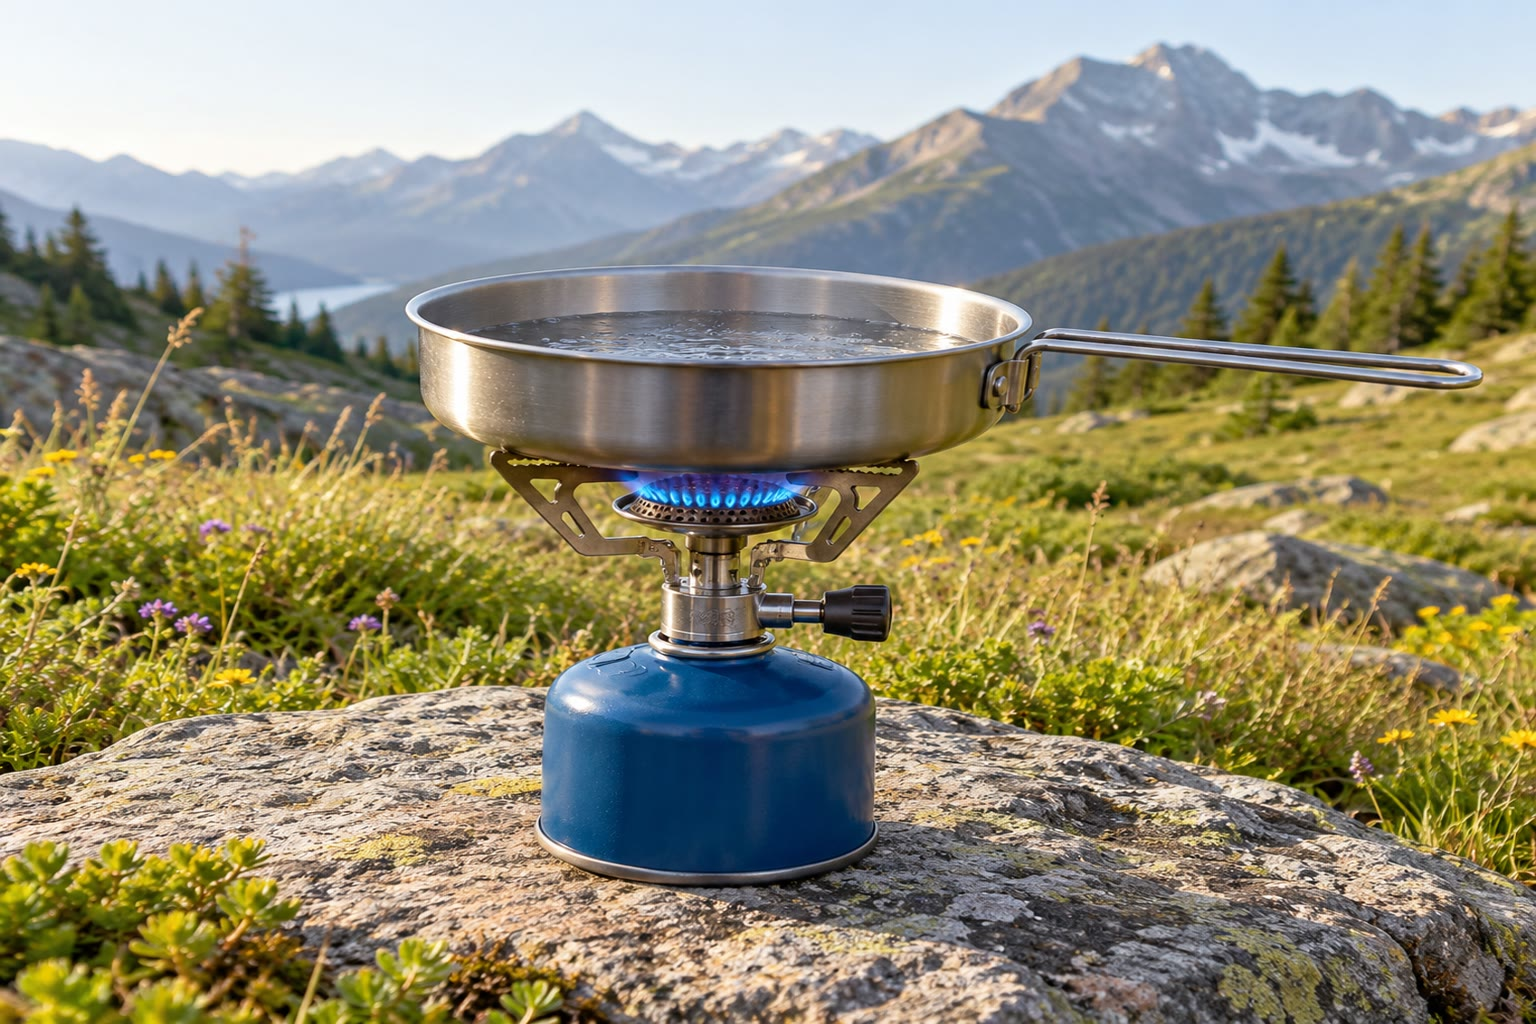
\includegraphics[width=0.6\linewidth]{images/book3/ai/b2-01-camping-stove.jpg}

{\small Un hornillo de camping: el butano del cartucho arde en el aire bajo
el cazo. El calor liberado por mol de butano, la parte que llega al
agua y la temperatura de la llama se calculan en el problema de fin de
semana de este capítulo.}
\end{omfigure}

\section{Magnitudes de reacción}

Un sistema cerrado en el que tiene lugar la única reacción $0 = \sum_i\nu_i\mathrm A_i$
se describe por su temperatura, su presión y su avance:
las cantidades son $n_i = n_{i,0} + \nu_i\xi$. Toda función de estado extensiva
del sistema, por ejemplo su entalpía, es entonces una función $H(T, p,
\xi)$, y su diferencial exacta es
\[
  \dd H = \left(\frac{\partial H}{\partial T}\right)_{p,\xi}\dd T
        + \left(\frac{\partial H}{\partial p}\right)_{T,\xi}\dd p
        + \left(\frac{\partial H}{\partial \xi}\right)_{T,p}\dd\xi .
\]

\begin{definition}[Magnitud de reacción, entalpía de reacción]\label{def:b2:reaction-enthalpy:reaction-quantity}
Para una función de estado extensiva $X$ de un sistema cerrado en el que
tiene lugar la reacción $0 = \sum_i\nu_i\mathrm A_i$, la \emph{magnitud de
reacción}\index{magnitud de reaccion@magnitud de reacción} es la derivada parcial
\[
  \Delta_r X = \left(\frac{\partial X}{\partial \xi}\right)_{T,p} ,
\]
la variación de $X$ por unidad de avance a temperatura y presión fijas, en
unidades de $X$ por mol. Para $X = H$ es la \emph{entalpía de
reacción}\index{entalpia de reaccion@entalpía de reacción} $\Delta_r H$, en \unit{kJ/mol}.
\end{definition}

\begin{remark}[Una derivada, no una diferencia]\label{rem:b2:reaction-enthalpy:operator}
El símbolo $\Delta_r$ es un operador: se aplica al estado del
sistema, que deja inalterado. Escribir la reacción de otro modo
(duplicando sus coeficientes) duplica $\Delta_r H$, de modo que una \omterm{def:b2:reaction-enthalpy:reaction-quantity}{magnitud de reacción} no
tiene sentido sin su ecuación. Cuando se usan las entalpías molares parciales
$\bar H_i = (\partial H/\partial n_i)_{T,p,n_j}$ de las especies
(\cref{ch:b2:chemical-potential}), $\Delta_r H = \sum_i\nu_i\bar H_i$, por
la regla de la cadena aplicada a $n_i = n_{i,0} + \nu_i\xi$.
\end{remark}

\begin{proposition}[Calor recibido a temperatura y presión constantes]\label{prop:b2:reaction-enthalpy:qp}
Cuando la reacción avanza de $\xi_1$ a $\xi_2$ en un sistema mantenido a
$T$ y $p$ constantes, el sistema recibe el calor
\[
  Q_p = \int_{\xi_1}^{\xi_2}\Delta_r H\,\dd\xi = \Delta_r H\,(\xi_2 - \xi_1)
\]
cuando $\Delta_r H$ no depende de $\xi$.
\end{proposition}

\begin{proof}
A $p$ constante (y, aquí, a presión exterior constante), el calor recibido
es la variación de entalpía, $Q_p = \Delta H$ (física). A $T$ y $p$ fijas
la diferencial de $H$ se reduce a $\dd H = \Delta_r H\,\dd\xi$; integrando
de $\xi_1$ a $\xi_2$ se obtiene el resultado.
\end{proof}

\begin{definition}[Exotérmica, endotérmica, atérmica]\label{def:b2:reaction-enthalpy:exothermic}
Una reacción es \emph{exotérmica}\index{exotermica@exotérmica} en un estado dado si
$\Delta_r H < 0$: llevada en sentido directo a $T$ y $p$ constantes, cede calor al
entorno. Es \emph{endotérmica}\index{endotermica@endotérmica} si $\Delta_r H >
0$, y \emph{atérmica}\index{atermica@atérmica} si $\Delta_r H = 0$.
\end{definition}

El calor de una reacción no depende, en general, de la composición:
para los gases perfectos y para los sólidos y líquidos puros, la entalpía de cada
especie no depende de lo que la rodea, y $\Delta_r H$ queda fijada
en cuanto lo está $T$.

\begin{proposition}[Sistemas ideales]\label{prop:b2:reaction-enthalpy:ideal}
En una mezcla de gases perfectos con fases condensadas puras, $\Delta_r H$
solo depende de la temperatura, y es igual a la \omterm{def:b2:reaction-enthalpy:standard-reaction-enthalpy}{entalpía estándar de
reacción} $\Delta_r H^\circ(T)$ definida más abajo. Para solutos en disolución
diluida la igualdad se cumple con buena aproximación.
\end{proposition}

\begin{proof}
En una mezcla de gases perfectos cada gas se comporta como si estuviera solo, con una entalpía
$n_iH_{m,i}(T)$ que no depende de $p$ (física: la entalpía de un
gas perfecto solo depende de $T$). Un sólido o un líquido puro tiene $H = n_iH_{m,i}(T,
p)$, y $(\partial H_m/\partial p)_T = V_m(1 - \alpha T)$ vale unos pocos
\unit{J/(mol.bar)} para una fase condensada, despreciable frente a \omterm{def:b2:reaction-enthalpy:reaction-quantity}{entalpías de
reacción} de decenas de \unit{kJ/mol}. Así, $H = \sum_in_iH_{m,i}(T)$, cuya
derivada respecto de $\xi$ es $\sum_i\nu_iH_{m,i}(T)$: solo depende de
$T$, y su valor es el que se calcula con cada especie en su
estado estándar.
\end{proof}

\section{Entalpías estándar de reacción y ley de Hess}

\begin{definition}[Magnitud estándar de reacción]\label{def:b2:reaction-enthalpy:standard-reaction-enthalpy}
La \emph{magnitud estándar de reacción}\index{magnitud estandar de reaccion@magnitud estándar de reacción}
$\Delta_r X^\circ(T) = \sum_i\nu_iX_{m,i}^\circ(T)$ es la \omterm{def:b2:reaction-enthalpy:reaction-quantity}{magnitud de reacción}
calculada con cada especie en su estado estándar a la temperatura $T$, siendo las
$X_{m,i}^\circ$ los valores molares estándar. Para $X = H$ es la
\emph{entalpía estándar de reacción}\index{entalpia estandar de reaccion@entalpía estándar de reacción}
$\Delta_r H^\circ(T)$; solo depende de $T$.
\end{definition}

Solo las diferencias de entalpía son medibles, así que se elige una referencia de una vez
por todas, como se eligió el electrodo de hidrógeno para los potenciales.

\begin{definition}[Estado estándar de referencia, entalpía estándar de formación]\label{def:b2:reaction-enthalpy:formation}
El \emph{estado estándar de referencia}\index{estado estandar de referencia@estado estándar de referencia} de un
elemento a la temperatura $T$ es su forma más estable a $T$ bajo $p^\circ$:
\ce{H2}, \ce{O2}, \ce{N2} y \ce{Cl2} como gases perfectos, el carbono como
grafito, el sodio como metal, el bromo como líquido (a \qty{298}{K}).
La \emph{entalpía estándar de formación}\index{entalpia estandar de formacion@entalpía estándar de formación}
$\Delta_f H^\circ$ de un compuesto es la \omterm{def:b2:reaction-enthalpy:standard-reaction-enthalpy}{entalpía estándar de reacción}
de su reacción de formación, la que produce un mol del
compuesto a partir de sus elementos en sus estados de referencia. Por construcción,
$\Delta_f H^\circ = 0$ para un elemento en su estado de referencia.
\end{definition}

\begin{example}[Reacciones de formación]\label{ex:b2:reaction-enthalpy:formation}
La reacción de formación del agua es \ce{H2(g) + 1/2O2(g) -> H2O(l)}, con
$\Delta_f H^\circ = \qty{-285.83}{kJ/mol}$ a \qty{298.15}{K}; la del
metano es \ce{C(s) + 2H2(g) -> CH4(g)}, $\Delta_f H^\circ =
\qty{-74.9}{kJ/mol}$; la del monóxido de nitrógeno, \ce{1/2N2(g) + 1/2O2(g) ->
NO(g)}, $\Delta_f H^\circ = \qty{+90.3}{kJ/mol}$: un compuesto \omterm{def:b2:reaction-enthalpy:exothermic}{endotérmico},
que los gases calientes de un motor producen a pesar de todo. Los coeficientes
fraccionarios no plantean problema: la reacción de formación es un recurso
contable, no un mecanismo.
% ledger: dfh:H2O-l, dfh:CH4_g, dfh:NO_g
\end{example}

\begin{theorem}[Ley de Hess]\label{thm:b2:reaction-enthalpy:hess}
Si una reacción es la suma, con coeficientes $\lambda_k$, de reacciones $k$,
su \omterm{def:b2:reaction-enthalpy:standard-reaction-enthalpy}{entalpía estándar de reacción} es la misma combinación de las de estas:
$\Delta_r H^\circ = \sum_k\lambda_k\Delta_r H_k^\circ$
(\emph{ley de Hess}\index{ley de Hess}). En particular, una \omterm{def:b2:reaction-enthalpy:standard-reaction-enthalpy}{entalpía estándar de reacción}
puede calcularse a lo largo de cualquier camino de reacciones que lleve de los
reactivos a los productos.
\end{theorem}

\begin{proof}
Cada $\Delta_r H_k^\circ = \sum_i\nu_{i,k}H_{m,i}^\circ$ es lineal en los
números estequiométricos. Si la reacción es $\sum_k\lambda_k$ veces las
reacciones $k$, sus números estequiométricos son $\nu_i = \sum_k\lambda_k
\nu_{i,k}$, y $\Delta_r H^\circ = \sum_i\nu_iH_{m,i}^\circ = \sum_k\lambda_k
\sum_i\nu_{i,k}H_{m,i}^\circ$. Detrás del álgebra está el primer principio: $H$ es una
función de estado, de modo que su variación entre los mismos estados inicial y final
no depende del camino.
\end{proof}

\begin{proposition}[Entalpía de reacción a partir de las entalpías de formación]\label{prop:b2:reaction-enthalpy:formation-sum}
$\Delta_r H^\circ(T) = \sum_i\nu_i\,\Delta_f H_i^\circ(T)$.
\end{proposition}

\begin{proof}
Tómese el camino que descompone los reactivos en sus elementos en sus
estados de referencia (lo inverso de sus reacciones de formación, con los
coeficientes $-\nu_i > 0$) y luego forma los productos a partir de los mismos elementos
(coeficientes $\nu_i > 0$). Los elementos se cancelan porque la ecuación está
ajustada, y la \omterm{thm:b2:reaction-enthalpy:hess}{ley de Hess} suma las entalpías.
\end{proof}

\begin{omfigure}
\begin{tikzpicture}[font=\small, >={Stealth}, y=0.0062cm]
  \draw[->] (0,-1000) -- (0,180) node[above] {$H^\circ$ (\unit{kJ/mol})};
  \foreach \y in {0,-200,-400,-600,-800,-1000} \draw (-0.08,\y) -- (0.08,\y) node[left=4pt] {$\y$};
  % levels
  \draw[very thick] (1.0,0) -- (4.6,0) node[right] {\ce{C(s) + 2H2(g) + 2O2(g)}};
  \draw[very thick, omDef] (1.0,-74.9) -- (4.6,-74.9);
  \node[right, omDef] at (4.6,-110) {\ce{CH4(g) + 2O2(g)}};
  \draw[very thick, omThm] (1.0,-965.2) -- (4.6,-965.2) node[right] {\ce{CO2(g) + 2H2O(l)}};
  % arrows
  \draw[->, omDef, thick] (1.6,0) -- (1.6,-74.9);
  \node[omDef, anchor=south west, font=\footnotesize] at (1.1,5) {$\Delta_f H^\circ(\ce{CH4}) = -74.9$};
  \draw[->, omThm, thick] (3.9,0) -- (3.9,-965.2);
  \node[right, omThm, align=left] at (3.95,-500) {$\Delta_f H^\circ(\ce{CO2})$\\ $+ 2\Delta_f H^\circ(\ce{H2O})$\\ $= -965.2$};
  \draw[->, thick] (2.75,-74.9) -- (2.75,-965.2);
  \node[left, align=right] at (2.7,-650) {$\Delta_r H^\circ$\\ $= -890.3$};
\end{tikzpicture}

{\small Niveles de entalpía para la combustión del metano a \qty{298.15}{K}.
Los elementos en sus estados de referencia son el cero. El metano está
\qty{74.9}{kJ/mol} por debajo de ellos, y los productos \qty{965.2}{kJ/mol} por debajo:
la entalpía de combustión es la diferencia, \qty{-890.3}{kJ/mol}, sea cual sea
el camino que siga realmente la llama.}
% ledger: dfh:CH4_g, dfh:CO2, dfh:H2O-l
\end{omfigure}

\begin{example}[Combustión del metano]\label{ex:b2:reaction-enthalpy:methane}
Para \ce{CH4(g) + 2O2(g) -> CO2(g) + 2H2O(l)},
$\Delta_r H^\circ = -393.51 + 2(-285.83) - (-74.87) - 0 =
\qty{-890.3}{kJ/mol}$ a \qty{298.15}{K}. El valor medido en un
calorímetro es \qty{-890.7}{kJ/mol}: la tabla y la llama concuerdan dentro de
la incertidumbre de los datos. Si el agua sale como vapor
($\Delta_f H^\circ = \qty{-241.83}{kJ/mol}$), $\Delta_r H^\circ =
\qty{-802.3}{kJ/mol}$: la diferencia, \qty{88.0}{kJ}, es la entalpía de
vaporización de dos moles de agua, que una caldera de condensación recupera
condensando sus humos.
% ledger: dfh:CO2, dfh:H2O-l, dfh:CH4_g, dch:CH4, dfh:H2O_g (computed in figdata/bachelor-2/thermo-data.py)
\end{example}

\begin{method}[Un ciclo de Hess]\label{met:b2:reaction-enthalpy:hess-cycle}
Para obtener la entalpía de una reacción que no puede medirse directamente:
\begin{enumerate}
  \item escríbase la reacción buscada con sus estados;
  \item búsquense reacciones de entalpía conocida (combustiones, formaciones) cuya
        combinación, con coeficientes $\lambda_k$, dé la reacción buscada;
  \item compruébese que toda especie ausente de la reacción buscada se cancela;
  \item súmense las entalpías con los mismos coeficientes.
\end{enumerate}
\end{method}

\begin{example}[Del carbono al monóxido de carbono]\label{ex:b2:reaction-enthalpy:co}
Al quemar carbono siempre se forma algo de dióxido de carbono, de modo que la entalpía de
\ce{C(s) + 1/2O2(g) -> CO(g)} no se mide directamente. Las dos combustiones
\ce{C(s) + O2(g) -> CO2(g)} ($\qty{-393.51}{kJ/mol}$) y \ce{CO(g) +
1/2O2(g) -> CO2(g)} ($\qty{-283.0}{kJ/mol}$, medida) sí se miden; la reacción buscada es
la primera menos la segunda: $\Delta_r H^\circ = -393.51 + 283.0 =
\qty{-110.5}{kJ/mol}$, la entalpía de formación del monóxido de carbono.
% ledger: dfh:CO2, dfh:CO_g
\end{example}

\begin{history}[Germain Henri Hess]
\begin{minipage}[t]{0.2\linewidth}\vspace{0pt}
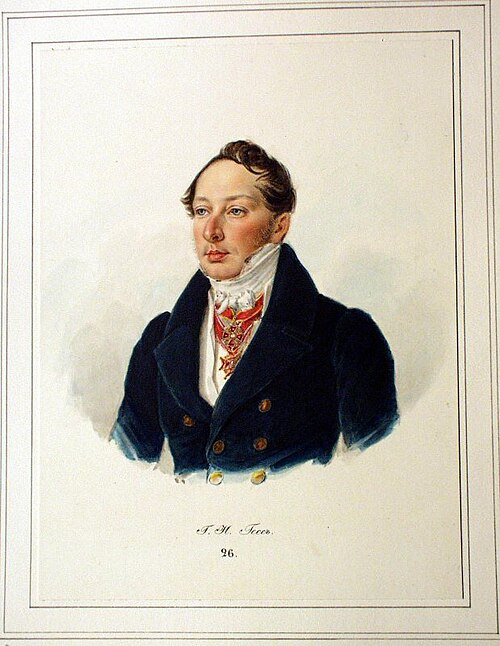
\includegraphics[width=\linewidth]{images/book3/hess.jpg}
\end{minipage}\hfill
\begin{minipage}[t]{0.76\linewidth}\vspace{0pt}
Germain Henri Hess (1802--1850), profesor de química en San
Petersburgo, midió los calores liberados al diluir o neutralizar ácido
sulfúrico en varias etapas, y halló en 1840 que el total no
dependía de las etapas seguidas: la ``ley de la suma constante de calores'', enunciada
antes que el propio primer principio de la termodinámica, que la explica.
(Retrato de I. I. Reimers, 1837--1838; CC BY-SA 4.0, Wikimedia Commons.)
\end{minipage}
\end{history}

\section{Cálculo de entalpías de reacción}

\subsection*{A partir de las entalpías de enlace}

Cuando falta la entalpía de formación de un compuesto, la energía de sus
enlaces da una estimación, en fase gaseosa.

\begin{definition}[Entalpía de disociación de enlace, entalpía media de enlace]\label{def:b2:reaction-enthalpy:bond-enthalpy}
La \emph{entalpía de disociación de enlace}\index{entalpia de disociacion de enlace@entalpía de disociación de enlace} de
un enlace A--B en una molécula gaseosa es la \omterm{def:b2:reaction-enthalpy:standard-reaction-enthalpy}{entalpía estándar de reacción} de la
ruptura de ese enlace en dos fragmentos gaseosos, \ce{AB(g) -> A(g) + B(g)}
para una molécula diatómica. Cuando una molécula tiene $n$ enlaces iguales, su
\emph{entalpía media de enlace}\index{entalpia media de enlace@entalpía media de enlace} es la entalpía
estándar de su atomización completa en átomos gaseosos dividida por $n$.
\end{definition}

Las entalpías de atomización son a su vez entalpías de formación: las de
los átomos gaseosos, menos la de la molécula. La tabla siguiente se ha
calculado de este modo.

\begin{omfigure}
\begin{tabular}{lrl}
\hline
enlace & entalpía (\unit{kJ/mol}) & obtenida de \\
\hline
H--H & 436 & \ce{H2}, disociación \\
O=O & 498 & \ce{O2}, disociación \\
N$\equiv$N & 945 & \ce{N2}, disociación \\
Cl--Cl & 243 & \ce{Cl2}, disociación \\
H--Cl & 432 & \ce{HCl}, disociación \\
C--H & 416 & \ce{CH4}, media de cuatro \\
N--H & 391 & \ce{NH3}, media de tres \\
O--H & 464 & \ce{H2O}, media de dos \\
C=O & 804 & \ce{CO2}, media de dos \\
C--C & 330 & \ce{C2H6}, con el C--H tomado del metano \\
C=C & 589 & \ce{C2H4}, con el C--H tomado del metano \\
\hline
\end{tabular}

\smallskip
{\small Entalpías de enlace a \qty{298.15}{K}, calculadas a partir de las \omterm{def:b2:reaction-enthalpy:formation}{entalpías
estándar de formación} de los átomos y moléculas gaseosos. Las dos últimas
líneas muestran el límite del método: un enlace C--H del etano no es exactamente
uno del metano, y el valor de C--C hereda la diferencia.}
% ledger: dfh:C_g, janaf:H, dfh:O_g, dfh:N_g, janaf:Cl, janaf:HCl, dfh:CH4_g, dfh:NH3_g, dfh:H2O_g, dfh:CO2, dfh:C2H6_g, dfh:C2H4_g (computed in figdata/bachelor-2/thermo-data.py)
\end{omfigure}

\begin{proposition}[Estimación a partir de las entalpías de enlace]\label{prop:b2:reaction-enthalpy:bond-estimate}
Para una reacción entre gases,
\[
  \Delta_r H^\circ \approx \sum(\text{entalpías de los enlaces rotos}) -
  \sum(\text{entalpías de los enlaces formados}).
\]
\end{proposition}

\begin{proof}
Sígase el camino que atomiza todos los reactivos (entalpía: los enlaces rotos)
y luego construye los productos a partir de los átomos (menos los enlaces formados). La \omterm{thm:b2:reaction-enthalpy:hess}{ley
de Hess} hace exacta la suma cuando cada entalpía de enlace es la del enlace en su
propia molécula; sustituirla por un valor medio tomado de otra molécula es la
aproximación.
\end{proof}

\begin{example}[Hidrogenación del eteno]\label{ex:b2:reaction-enthalpy:hydrogenation}
En \ce{C2H4(g) + H2(g) -> C2H6(g)} se rompen un C=C y un H--H, que se
sustituyen por un C--C y dos C--H. Con la tabla: $589 + 436 - 330 - 2
\times 416 = \qty{-137}{kJ/mol}$; a partir de las entalpías de formación el valor es
\qty{-136.3}{kJ/mol}. La concordancia es buena aquí porque los valores de C--C
y C=C de la tabla se obtuvieron de estas mismas moléculas; para una molécula distinta
de las de la tabla, un error de 10 a \qty{30}{kJ/mol} es habitual.
% ledger: dfh:C2H4_g, dfh:C2H6_g
\end{example}

\subsection*{Entalpías reticulares: el ciclo de Born--Haber}

\begin{definition}[Entalpía reticular]\label{def:b2:reaction-enthalpy:lattice-enthalpy}
La \emph{entalpía reticular}\index{entalpia reticular@entalpía reticular} de un cristal iónico es
la \omterm{def:b2:reaction-enthalpy:standard-reaction-enthalpy}{entalpía estándar de reacción} de su disociación en iones gaseosos: para
el cloruro de sodio, \ce{NaCl(s) -> Na+(g) + Cl-(g)}. Es positiva y
mide la cohesión del cristal.
\end{definition}

No puede medirse directamente, pero un ciclo a través de los elementos la da
a partir de magnitudes medibles: la entalpía de formación del cristal, la
atomización de los elementos, la energía de ionización del metal y la
afinidad electrónica del no metal (ambas definidas en el volumen del primer año).

\begin{omfigure}
\begin{tikzpicture}[font=\small, >={Stealth}, y=0.0058cm]
  \def\lw{5.0}
  % levels (kJ/mol relative to Na(s) + 1/2 Cl2(g))
  \draw[thick] (0,0) -- (\lw,0) node[right] {\ce{Na(s) + 1/2Cl2(g)}};
  \draw[thick] (0,107.5) -- (\lw,107.5) node[right] {\ce{Na(g) + 1/2Cl2(g)}};
  \draw[thick] (0,228.8) -- (\lw,228.8) node[right] {\ce{Na(g) + Cl(g)}};
  \draw[thick] (0,724.6) -- (\lw,724.6) node[right] {\ce{Na+(g) + e- + Cl(g)}};
  \draw[thick] (0,376.1) -- (\lw,376.1) node[right] {\ce{Na+(g) + Cl-(g)}};
  \draw[thick] (0,-411.1) -- (\lw,-411.1) node[right] {\ce{NaCl(s)}};
  % the path through the elements, on the left
  \draw[->, omDef] (0.4,0) -- (0.4,107.5);
  \node[omDef, left, font=\footnotesize] at (0.35,53) {sublimación $107.5$};
  \draw[->, omDef] (0.4,107.5) -- (0.4,228.8);
  \node[omDef, left, font=\footnotesize] at (0.35,168) {$\tfrac12$ disociación $121.3$};
  \draw[->, omDef] (0.4,228.8) -- (0.4,724.6);
  \node[omDef, left, font=\footnotesize] at (0.35,480) {ionización de Na $495.8$};
  \draw[->, omThm] (1.4,724.6) -- (1.4,376.1);
  \node[omThm, right, font=\footnotesize] at (1.45,560) {captura electrónica $-348.6$};
  \draw[->, omProp] (2.3,0) -- (2.3,-411.1);
  \node[omProp, left, font=\footnotesize] at (2.25,-205) {formación $-411.1$};
  % the lattice enthalpy, the only unknown
  \draw[->, thick] (3.6,-411.1) -- (3.6,376.1);
  \node[right, font=\footnotesize] at (3.65,-205) {entalpía reticular $787$};
\end{tikzpicture}

{\small El ciclo de Born--Haber del cloruro de sodio a \qty{298}{K}
(\unit{kJ/mol}). Subir del cristal a los iones gaseosos por la
\omterm{def:b2:reaction-enthalpy:lattice-enthalpy}{entalpía reticular}, o dar la vuelta por los elementos, lleva al mismo nivel: la
\omterm{def:b2:reaction-enthalpy:lattice-enthalpy}{entalpía reticular} es la única incógnita del ciclo.}
% ledger: dfh:NaCl_cr, dfh:Na_g, janaf:Cl, ie:Na, ea:Cl
\end{omfigure}

\begin{method}[El ciclo de Born--Haber]\label{met:b2:reaction-enthalpy:born-haber}
\begin{enumerate}
  \item Desde los elementos en sus estados de referencia, trácense dos caminos: uno
        hasta el cristal (formación) y otro hasta los iones gaseosos (sublimación del
        metal, atomización del no metal, ionización, captura
        electrónica).
  \item Ciérrese el ciclo con la \omterm{def:b2:reaction-enthalpy:lattice-enthalpy}{entalpía reticular}, del cristal hasta
        los iones gaseosos.
  \item Escríbase que la suma de las entalpías a lo largo del ciclo es nula, y
        despéjese la incógnita. Las energías de ionización y las afinidades electrónicas
        se tabulan en eV por átomo: multiplíquese por $N_A e = \qty{96.485}{kJ/(mol.eV)}$.
\end{enumerate}
\end{method}

\begin{example}[Cloruro de sodio]\label{ex:b2:reaction-enthalpy:nacl}
$\Delta_{\text{ret}}H^\circ = 411.1 + 107.5 + 121.3 + 495.8 - 348.6 =
\qty{787}{kJ/mol}$. La energía de ionización y la afinidad electrónica son
energías a \qty{0}{K}; sus correcciones a \qty{298}{K} ($+\tfrac52RT$
para cada una) se cancelan entre las dos etapas. Un modelo de cristal de cargas puntuales
da un valor parecido, y por eso se dice que el cloruro de sodio es iónico.
% ledger: dfh:NaCl_cr, dfh:Na_g, janaf:Cl, ie:Na, ea:Cl (computed in figdata/bachelor-2/thermo-data.py)
\end{example}

\section{Entalpías de reacción y temperatura}

Las tablas dan $\Delta_f H^\circ$ a \qty{298.15}{K}. Un reactor funciona a
\qty{700}{K}, una llama a \qty{2000}{K}: ¿cómo varía $\Delta_r H^\circ$
con la temperatura?

\begin{theorem}[Ley de Kirchhoff]\label{thm:b2:reaction-enthalpy:kirchhoff}
\[
  \frac{\dd\Delta_r H^\circ}{\dd T} = \Delta_r C_p^\circ =
  \sum_i\nu_i C_{p,m,i}^\circ ,
\]
de modo que $\Delta_r H^\circ(T_2) = \Delta_r H^\circ(T_1) + \int_{T_1}^{T_2}
\Delta_r C_p^\circ\,\dd T$ (\emph{ley de Kirchhoff}\index{ley de Kirchhoff}),
en ausencia de cambio de estado entre $T_1$ y $T_2$.
\end{theorem}

\begin{proof}
Con cada especie en su estado estándar, $H^\circ(T, \xi) = \sum_in_i
H^\circ_{m,i}(T)$ es una función de dos variables cuyas derivadas parciales
segundas son continuas; por el teorema de Schwarz, conmutan:
\[
  \frac{\dd\Delta_r H^\circ}{\dd T} = \frac{\partial}{\partial T}
  \frac{\partial H^\circ}{\partial\xi} = \frac{\partial}{\partial\xi}
  \frac{\partial H^\circ}{\partial T} = \frac{\partial}{\partial\xi}
  \sum_in_iC^\circ_{p,m,i} = \sum_i\nu_iC^\circ_{p,m,i}.
\]
Integrando entre $T_1$ y $T_2$ se obtiene la segunda forma. Un cambio de
estado de una especie dentro del intervalo añade su entalpía de transición,
con el número estequiométrico.
\end{proof}

\begin{example}[Síntesis del amoníaco en caliente]\label{ex:b2:reaction-enthalpy:kirchhoff}
Para \ce{N2(g) + 3H2(g) -> 2NH3(g)}, $\Delta_r H^\circ(298) =
\qty{-91.9}{kJ/mol}$ y, con las capacidades caloríficas a \qty{298}{K},
$\Delta_r C_p^\circ = 2(35.65) - 29.12 - 3(28.84) =
\qty{-44.3}{J/(K.mol)}$. Tomada como constante, da $\Delta_r
H^\circ(700) = -91.9 - 0.0443 \times 402 = \qty{-109.7}{kJ/mol}$. Las tablas,
que siguen las capacidades caloríficas a medida que crecen con la temperatura, dan
\qty{-105.2}{kJ/mol}: la estimación con $C_p$ constante se desvía un 4\,\%, un
precio razonable para un cálculo de una línea. En \qty{400}{K}, la \omterm{def:b2:reaction-enthalpy:reaction-quantity}{entalpía de
reacción} varía en torno a una séptima parte.
% ledger: dfh:NH3_g, cp:NH3_g.298, cp:N2_g.298, cp:H2_g.298, janafdfH:NH3.700 (computed in figdata/bachelor-2/thermo-data.py)
\end{example}

\section{Reacciones adiabáticas y calorimetría}

\subsection*{Temperatura de llama}

En una llama la reacción es rápida y el calor no tiene tiempo de salir: los
gases se calientan a sí mismos.

\begin{definition}[Temperatura adiabática de llama]\label{def:b2:reaction-enthalpy:flame-temperature}
La \emph{temperatura adiabática de llama}\index{temperatura adiabatica de llama@temperatura adiabática de llama}
de un combustible es la temperatura que alcanzan los productos de su
combustión completa cuando la reacción tiene lugar a presión constante, sin
ningún intercambio de calor, a partir de reactivos a \qty{298}{K}.
\end{definition}

\begin{proposition}[Cálculo de una temperatura de llama]\label{prop:b2:reaction-enthalpy:flame}
Si la reacción avanza en $\xi$ a partir de reactivos a $T_0$ y el sistema final
tiene una capacidad calorífica $C_p(T)$, la temperatura final $T_f$ cumple
\[
  \xi\,\Delta_r H^\circ(T_0) + \int_{T_0}^{T_f}C_p(T)\,\dd T = 0 .
\]
\end{proposition}

\begin{proof}
Adiabática y a presión constante, la transformación tiene $\Delta H =
Q_p = 0$. Como $H$ es una función de estado, cualquier camino entre los mismos estados
inicial y final da el mismo $\Delta H$. Tómese el camino de
la figura siguiente: primero la reacción a $T_0$, con
$\Delta H_1 = \xi\Delta_r H^\circ(T_0)$ (\cref{prop:b2:reaction-enthalpy:qp},
con comportamiento ideal); después el calentamiento del sistema final de $T_0$ a
$T_f$, $\Delta H_2 = \int C_p\,\dd T$. Su suma es nula.
\end{proof}

\begin{omfigure}
\begin{tikzpicture}[font=\small, >={Stealth}]
  \draw[->] (0,0) -- (6.2,0) node[right] {avance $\xi$};
  \draw[->] (0,0) -- (0,3.6) node[above] {temperatura $T$};
  \fill (0.6,0.6) circle (2pt) node[below left] {reactivos, $T_0$};
  \fill (5.2,0.6) circle (2pt) node[below] {productos, $T_0$};
  \fill (5.2,3.0) circle (2pt) node[right] {productos, $T_f$};
  \draw[->, thick, omDef] (0.7,0.6) -- (5.1,0.6);
  \node[omDef, above, font=\footnotesize] at (3.15,0.64) {$\Delta H_1 = \xi\,\Delta_r H^\circ(T_0) < 0$};
  \draw[->, thick, omThm] (5.2,0.7) -- (5.2,2.9);
  \node[omThm, right, align=left] at (5.25,1.8) {$\Delta H_2 = \int_{T_0}^{T_f} C_p\,\dd T$};
  \draw[->, thick, dashed] (0.75,0.75) -- (5.05,2.92);
  \node[above left, align=center] at (2.6,1.75) {llama real:\\ $\Delta H = 0$};
\end{tikzpicture}

{\small La llama adiabática (en trazo discontinuo) y un camino equivalente en dos
etapas: reacción a temperatura constante y luego calentamiento de los productos.
Como $H$ es una función de estado, las dos variaciones de entalpía de las etapas suman
cero.}
\end{omfigure}

\begin{method}[Temperatura de llama]\label{met:b2:reaction-enthalpy:flame-temperature}
\begin{enumerate}
  \item Escríbase la combustión completa de un mol de combustible; en aire, añádanse
        el nitrógeno y el argón que acompañan al oxígeno (también se
        calientan); tómese el agua como vapor.
  \item Calcúlese $q = -\Delta_r H^\circ(T_0)$ por mol de combustible.
  \item O bien se toma una capacidad calorífica $C_p$ constante de los productos:
        $T_f = T_0 + q/C_p$; o bien se busca $T_f$ tal que la suma de los
        incrementos tabulados $n_i[H^\circ_{m,i}(T_f) - H^\circ_{m,i}(T_0)]$
        sea igual a $q$, por interpolación.
\end{enumerate}
\end{method}

\begin{omfigure}
\begin{tikzpicture}
\begin{axis}[
  width=0.8\linewidth, height=6.2cm, xmin=300, xmax=3000, ymin=0, ymax=3200,
  axis x line=bottom, axis y line=left, xlabel={$T$ (K)},
  ylabel={$H(T) - H(\qty{298}{K})$ de los productos (kJ)},
  xtick={500,1000,1500,2000,2500,3000},
  tick label style={font=\small}, label style={font=\small}, clip=false,
  legend style={font=\scriptsize, draw=none, at={(0.5,1.03)}, anchor=south}, legend columns=2]
\addplot[omDef, very thick] table[x=T, y=H] {figdata/out/bachelor-2-flame-temperature-butane.dat};
\addplot[omThm, very thick] table[x=T, y=H] {figdata/out/bachelor-2-flame-temperature-methane.dat};
\legend{1 mol de butano en aire, 1 mol de metano en aire}
\draw[omDef, dashed] (axis cs:300,2657.6) -- (axis cs:3000,2657.6);
\node[omDef, anchor=south east, font=\scriptsize] at (axis cs:2350,2657.6) {$-\Delta_r H^\circ = \qty{2657.6}{kJ}$};
\draw[omDef, dotted] (axis cs:2401,0) -- (axis cs:2401,2657.6);
\fill[omDef] (axis cs:2401,2657.6) circle (1.5pt);
\node[omDef, anchor=north west, font=\scriptsize] at (axis cs:2420,2620) {\qty{2401}{K}};
\draw[omThm, dashed] (axis cs:300,802.3) -- (axis cs:3000,802.3);
\node[omThm, anchor=south west, font=\scriptsize] at (axis cs:320,802.3) {$-\Delta_r H^\circ = \qty{802.3}{kJ}$};
\draw[omThm, dotted] (axis cs:2329,0) -- (axis cs:2329,802.3);
\fill[omThm] (axis cs:2329,802.3) circle (1.5pt);
\node[omThm, anchor=north west, font=\scriptsize] at (axis cs:2350,760) {\qty{2329}{K}};
\end{axis}
\end{tikzpicture}

{\small Entalpía necesaria para calentar desde \qty{298}{K} los productos de combustión de un mol de
combustible (dióxido de carbono, vapor de agua y el nitrógeno y el argón del aire),
según las entalpías tabuladas. Cada curva alcanza el calor
liberado por su combustión a la \omterm{def:b2:reaction-enthalpy:flame-temperature}{temperatura adiabática de llama}: unos
\qty{2400}{K} para el butano y \qty{2330}{K} para el metano.}
% ledger: janafH:CO2.2400, janafH:H2O.2400, janafH:N2.2400, janafH:Ar.2400, air:N2, air:O2, air:Ar (computed in figdata/bachelor-2/flame-temperature.py)
\end{omfigure}

Las temperaturas calculadas son cotas superiores. Por encima de unos \qty{2000}{K},
el dióxido de carbono y el agua empiezan a disociarse en monóxido de carbono,
hidrógeno, oxígeno y radicales; estas reacciones \omterm{def:b2:reaction-enthalpy:exothermic}{endotérmicas} recuperan parte
del calor, y una llama real de butano en aire es claramente más fría
de lo calculado. En oxígeno puro no hay nitrógeno que calentar y la llama es
mucho más caliente, y por eso los soldadores queman etino con oxígeno y no con
aire.

\subsection*{Calorimetría}

\begin{proposition}[Volumen constante y presión constante]\label{prop:b2:reaction-enthalpy:bomb}
En un recipiente cerrado de acero (una bomba calorimétrica) el calor medido es $Q_V =
\Delta U$, y para gases perfectos y fases condensadas
\[
  \Delta_r H = \Delta_r U + \Delta\nu_{\text{gas}}\,RT ,
\]
donde $\Delta\nu_{\text{gas}}$ es la suma de los números estequiométricos de
las especies gaseosas.
\end{proposition}

\begin{proof}
$H = U + pV$, y $\Delta_r H = \Delta_r U + \partial(pV)/\partial\xi$ a
$T$ fija. El $pV$ de las fases condensadas es despreciable, y para los
gases $pV = n_{\text{gas}}RT$ con $n_{\text{gas}} = n_{\text{gas},0} +
\Delta\nu_{\text{gas}}\xi$, cuya derivada respecto de $\xi$ es
$\Delta\nu_{\text{gas}}RT$.
\end{proof}

\begin{omfigure}
\begin{tikzpicture}[font=\small, >={Stealth}, scale=1.0]
  % outer insulated jacket
  \draw[thick, fill=gray!8] (-2.6,-0.2) rectangle (2.6,4.4);
  \draw[thick, fill=white] (-2.3,0.1) rectangle (2.3,4.1);
  % water bath
  \fill[omDef!12] (-2.3,0.1) rectangle (2.3,3.4);
  \draw[omDef!60] (-2.3,3.4) -- (2.3,3.4);
  % bomb
  \draw[very thick, fill=gray!35] (-0.75,0.5) rectangle (0.75,2.6);
  \draw[very thick, fill=gray!55] (-0.9,2.6) rectangle (0.9,2.85);
  \draw[thick] (-0.3,1.0) -- (-0.3,1.9) (0.3,1.0) -- (0.3,1.9);
  \draw[thick, fill=orange!50] (-0.3,0.95) rectangle (0.3,1.05);
  \draw[red!70!black, thick, decorate, decoration={zigzag, amplitude=1pt, segment length=3pt}] (-0.3,1.9) -- (0.3,1.9);
  % wires
  \draw (-0.3,2.85) -- (-0.3,4.7) (0.3,2.85) -- (0.3,4.7);
  % stirrer and thermometer
  \draw[thick] (1.6,0.6) -- (1.6,4.7);
  \draw[thick, fill=gray!40] (1.35,0.55) rectangle (1.85,0.75);
  \pic[transform shape] at (-1.6,0.4) {thermometer};
  % labels
  \draw (-0.75,1.6) -- (-3.3,1.6) node[left] {bomba de acero, \ce{O2} a 30 bar};
  \draw (0,1.0) -- (-3.3,0.6) node[left] {muestra en su cápsula};
  \draw (0,1.9) -- (-3.3,2.6) node[left] {hilo de ignición};
  \draw (1.0,3.0) -- (3.3,3.0) node[right] {baño de agua};
  \draw (1.6,3.9) -- (3.3,4.3) node[right] {agitador};
  \draw (-1.6,3.4) -- (-3.3,3.6) node[left] {termómetro};
  \draw (2.45,0.3) -- (3.3,0.5) node[right] {camisa aislante};
\end{tikzpicture}

{\small Una bomba calorimétrica. La muestra arde a volumen constante en
oxígeno a presión; el calor pasa a la bomba y al agua agitada,
cuyo aumento de temperatura se lee en el termómetro. La capacidad
calorífica del calorímetro se determina antes quemando un patrón de energía conocida.}
\end{omfigure}

\begin{method}[Calorimetría]\label{met:b2:reaction-enthalpy:calorimetry}
\begin{enumerate}
  \item Calíbrese: quémese una masa de un patrón de energía de combustión conocida
        (o hágase pasar una energía eléctrica conocida), léase el aumento de temperatura
        $\Delta T$ y dedúzcase la capacidad calorífica $C$ de todo el
        calorímetro (agua y recipiente, su ``equivalente en agua'').
  \item Quémese la muestra y léase $\Delta T'$: el calor liberado es $C\,\Delta
        T'$, luego $\Delta_r U = -C\Delta T'/\xi$ a volumen constante.
  \item Corríjase a $\Delta_r H$ con $\Delta\nu_{\text{gas}}RT$; en un calorímetro
        abierto (a presión constante), $\Delta_r H = -C\Delta T'/\xi$
        directamente.
\end{enumerate}
\end{method}

\begin{example}[Una medida en la bomba]\label{ex:b2:reaction-enthalpy:bomb}
Para la combustión del butano con agua líquida, $\Delta\nu_{\text{gas}} = 4
- 1 - 6.5 = -3.5$, luego $\Delta_r U = \Delta_r H + 3.5RT = -2877.6 + 8.7 =
\qty{-2868.9}{kJ/mol}$: la corrección es de unas pocas partes por mil, mayor
que la incertidumbre de una buena medida en la bomba, así que nunca se omite.
% ledger: dfh:C4H10_g, dfh:CO2, dfh:H2O-l (computed in figdata/bachelor-2/thermo-data.py)
\end{example}

\begin{history}[Bombas calorimétricas, 1881]
\begin{minipage}[t]{0.2\linewidth}\vspace{0pt}
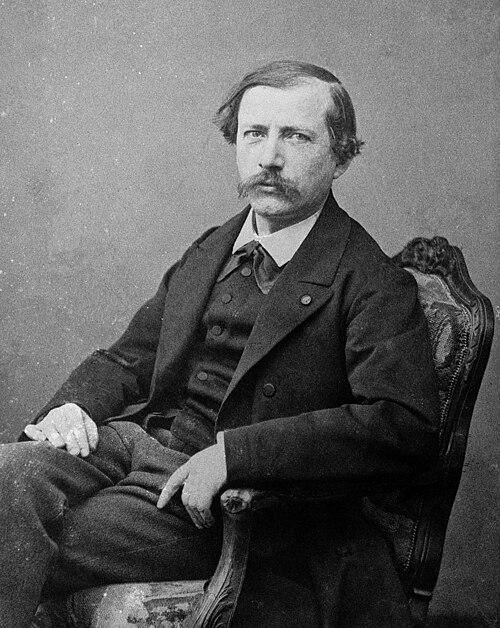
\includegraphics[width=\linewidth]{images/book3/berthelot.jpg}
\end{minipage}\hfill
\begin{minipage}[t]{0.76\linewidth}\vspace{0pt}
Marcellin Berthelot (1827--1907) quemó compuestos orgánicos en oxígeno
comprimido dentro de un recipiente cerrado de acero forrado de platino, de modo que la
combustión fuera completa y nada escapara: la bomba calorimétrica, todavía
el instrumento de referencia para los calores de combustión. Acuñó también las palabras
\omterm{def:b2:reaction-enthalpy:exothermic}{exotérmico} y \omterm{def:b2:reaction-enthalpy:exothermic}{endotérmico}. (Fotografía: dominio público, Wikimedia
Commons.)
\end{minipage}
\end{history}

\section{Ejercicios}

\begin{exercise}[$\star$]\label{exo:b2:reaction-enthalpy:1}
Con las \omterm{def:b2:reaction-enthalpy:formation}{entalpías estándar de formación} del capítulo, calcúlese
$\Delta_r H^\circ$ a \qty{298}{K} de la combustión del propano,
\ce{C3H8(g) + 5O2(g) -> 3CO2(g) + 4H2O(l)}, sabiendo que $\Delta_f
H^\circ(\ce{C3H8}, \text{g}) = \qty{-104.7}{kJ/mol}$. ¿Es la reacción
\omterm{def:b2:reaction-enthalpy:exothermic}{exotérmica}?
% ledger: dfh:C3H8_g
\end{exercise}

\begin{exercise}[$\star$]\label{exo:b2:reaction-enthalpy:2}
Calcúlese el calor liberado al quemar \qty{1.00}{kg} de metano (agua
formada líquida) y \qty{1.00}{kg} de dihidrógeno, \ce{H2(g) + 1/2O2(g) ->
H2O(l)}. ¿Qué combustible da más calor por kilogramo?
\end{exercise}

\begin{exercise}[$\star$]\label{exo:b2:reaction-enthalpy:3}
Una bomba calorimétrica da $\Delta_r U = \qty{-3264}{kJ/mol}$ para el benceno
líquido que arde según \ce{C6H6(l) + 15/2O2(g) -> 6CO2(g) + 3H2O(l)} a
\qty{298}{K}. Calcúlese $\Delta_r H$.
\end{exercise}

\begin{exercise}[$\star$]\label{exo:b2:reaction-enthalpy:4}
Dados $\Delta_r H^\circ = \qty{-393.5}{kJ/mol}$ para \ce{C(s) + O2(g) ->
CO2(g)} y $\Delta_r H^\circ = \qty{-283.0}{kJ/mol}$ para \ce{CO(g) +
1/2O2(g) -> CO2(g)}, calcúlese la entalpía de \ce{CO2(g) + C(s) -> 2CO(g)},
la reacción que tiene lugar en el coque caliente de un alto horno.
\end{exercise}

\begin{exercise}[$\star\star$]\label{exo:b2:reaction-enthalpy:5}
Estímese con las entalpías de enlace del capítulo la entalpía de
\ce{CH4(g) + Cl2(g) -> CH3Cl(g) + HCl(g)}, tomando \qty{350}{kJ/mol} para
C--Cl. Calcúlese después la misma magnitud a partir de las entalpías de formación,
sabiendo que $\Delta_f H^\circ(\ce{CH3Cl}, \text{g}) = \qty{-83.7}{kJ/mol}$, y
coméntese la diferencia.
% ledger: dfh:CH3Cl_g
\end{exercise}

\begin{exercise}[$\star\star$]\label{exo:b2:reaction-enthalpy:6}
La entalpía estándar de vaporización del agua a \qty{298}{K} es
$\Delta_f H^\circ(\ce{H2O}, \text{g}) - \Delta_f H^\circ(\ce{H2O},
\text{l})$. Calcúlese. Con $C_{p,m}^\circ = \qty{75.35}{J/(K.mol)}$ para
el líquido y \qty{33.59}{J/(K.mol)} para el vapor, ambas tomadas como
constantes, estímese a \qty{400}{K} (agua sobrecalentada a presión)
y compárese con las tablas, que dan $\Delta_f H^\circ =
\qty{-282.59}{kJ/mol}$ para el líquido y \qty{-242.85}{kJ/mol} para el
vapor a \qty{400}{K}.
% ledger: cp:H2O_l.298, cp:H2O_g.298, janafdfH:H2O_l.400, janafdfH:H2O_g.400
\end{exercise}

\begin{exercise}[$\star\star$]\label{exo:b2:reaction-enthalpy:7}
Mediante un ciclo de Born--Haber, calcúlese la \omterm{def:b2:reaction-enthalpy:lattice-enthalpy}{entalpía reticular} del cloruro
de potasio a partir de: $\Delta_f H^\circ(\ce{KCl}, \text{s}) = \qty{-436.7}{kJ/mol}$,
sublimación del potasio \qty{89.0}{kJ/mol}, energía de ionización del
potasio \qty{4.341}{eV}, $\Delta_f H^\circ(\ce{Cl}, \text{g}) =
\qty{121.3}{kJ/mol}$, afinidad electrónica del cloro \qty{3.613}{eV}. ¿Por qué
es menor que la del cloruro de sodio?
% ledger: dfh:KCl_cr, dfh:K_g, ie:K, janaf:Cl, ea:Cl
\end{exercise}

\begin{exercise}[$\star\star$]\label{exo:b2:reaction-enthalpy:8}
Un calorímetro de vaso aislado se calibra haciendo pasar \qty{2.00}{kJ} de
energía eléctrica, que eleva su temperatura en \qty{0.418}{K}. Después
se mezclan en él \qty{50.0}{mL} de ácido clorhídrico de \qty{1.00}{mol/L}
con \qty{50.0}{mL} de disolución de hidróxido de sodio de \qty{1.10}{mol/L},
ambas a la misma temperatura inicial: la temperatura sube
\qty{0.583}{K}. Calcúlese la entalpía de \ce{H3O+(aq) + OH-(aq) ->
2H2O(l)}.
\end{exercise}

\begin{exercise}[$\star\star$]\label{exo:b2:reaction-enthalpy:9}
El octano, modelo de la gasolina, tiene $\Delta_f H^\circ(\text{l}) =
\qty{-250.3}{kJ/mol}$. Calcúlense la entalpía de su combustión (agua
líquida), el calor liberado por kilogramo y la masa de dióxido de carbono
emitida por megajulio. Compárese con el metano.
% ledger: dfh:C8H18
\end{exercise}

\begin{exercise}[$\star\star\star$]\label{exo:b2:reaction-enthalpy:10}
Calcúlese la \omterm{def:b2:reaction-enthalpy:flame-temperature}{temperatura adiabática de llama} del metano que arde en la
cantidad estequiométrica de oxígeno puro, con capacidades caloríficas constantes (las
del capítulo a \qty{298}{K}: \ce{CO2} 37.13, \ce{H2O(g)}
\qty{33.59}{J/(K.mol)}). Compárese con el resultado en aire,
\qty{2780}{K} con la misma aproximación. ¿Por qué la llama real en oxígeno es
mucho más fría de lo que dice este cálculo?
% ledger: cp:CO2_g.298, cp:H2O_g.298
\end{exercise}

\begin{exercise}[$\star\star\star$]\label{exo:b2:reaction-enthalpy:11}
La capacidad calorífica de un gas se escribe a menudo $C_{p,m}^\circ = a + bT$. Para
la síntesis del amoníaco, tómense $\Delta_r a = \qty{-60.5}{J/(K.mol)}$ y
$\Delta_r b = \qty{0.0540}{J/(K^2.mol)}$ (ajustados a las tablas entre
\qty{300}{K} y \qty{800}{K}). Intégrese la \omterm{thm:b2:reaction-enthalpy:kirchhoff}{ley de Kirchhoff} de
\qty{298}{K} a \qty{700}{K} y compárese con el valor de las tablas,
\qty{-105.2}{kJ/mol}, y con la estimación con $C_p$ constante.
\end{exercise}

\begin{exercise}[$\star\star\star$]\label{exo:b2:reaction-enthalpy:12}
El monóxido de nitrógeno se forma en los motores según \ce{N2(g) + O2(g) -> 2NO(g)}.
Calcúlese su \omterm{def:b2:reaction-enthalpy:standard-reaction-enthalpy}{entalpía estándar de reacción} a \qty{298}{K}. Demuéstrese que, si
$\Delta_r C_p^\circ$ es pequeña, la reacción absorbe aproximadamente el mismo calor a
\qty{2000}{K}; con las capacidades caloríficas de las tablas a \qty{298}{K}
(\ce{NO} \qty{29.85}{J/(K.mol)}, \ce{N2} 29.12, \ce{O2}
\qty{29.38}{J/(K.mol)}), estímese la variación entre
\qty{298}{K} y \qty{2000}{K}. Explíquese por qué una reacción \omterm{def:b2:reaction-enthalpy:exothermic}{endotérmica} puede
ser un problema precisamente en las llamas más calientes.
% ledger: dfh:NO_g, cp:NO_g.298, cp:N2_g.298, cp:O2_g.298
\end{exercise}

\section{Problema: el cartucho de gas de camping}

\begin{problem}[{Problema de fin de semana --- la energía del butano, una medida en
una bomba calorimétrica, el agua calentada en un cazo y la temperatura de la
llama}]
\label{pb:b2:reaction-enthalpy:1}
Un hornillo de camping quema el butano de un cartucho que contiene \qty{230}{g}.
Datos a \qty{298}{K} ($\Delta_f H^\circ$ en \unit{kJ/mol}): \ce{C4H10(g)}
$-125.6$, \ce{CO2(g)} $-393.51$, \ce{H2O(l)} $-285.83$, \ce{H2O(g)}
$-241.83$. Masas molares: \ce{C4H10} \qty{58.12}{g/mol}, \ce{H2O}
\qty{18.02}{g/mol}. Capacidad calorífica del agua líquida
\qty{75.35}{J/(K.mol)}. Aire seco: \qty{20.95}{\percent} de \ce{O2},
\qty{78.08}{\percent} de \ce{N2} y \qty{0.93}{\percent} de \ce{Ar} en volumen. $R = \qty{8.314}{J/(K.mol)}$.
% ledger: dfh:C4H10_g, dfh:CO2, dfh:H2O-l, dfh:H2O_g, cp:H2O_l.298, air:O2, air:N2, air:Ar

\medskip
\noindent\textbf{Parte I --- El combustible.}
\begin{enumerate}
  \item Escríbase la combustión completa del butano, con el agua formada líquida,
        para un mol de butano.
  \item Calcúlese su \omterm{def:b2:reaction-enthalpy:standard-reaction-enthalpy}{entalpía estándar de reacción} a \qty{298}{K}.
  \item Calcúlese de nuevo con el agua formada como vapor, y explíquese la
        diferencia.
  \item Calcúlese el calor liberado por gramo de butano en cada caso.
  \item ¿Cuál de los dos valores describe un hornillo de camping, cuya agua
        sale de la llama como vapor?
  \item ¿Qué calor puede liberar todo el cartucho en el hornillo?
\end{enumerate}

\medskip
\noindent\textbf{Parte II --- Una medida.}
Se quema una muestra de \qty{0.500}{g} de butano en una bomba calorimétrica cuya
capacidad calorífica es \qty{10.00}{kJ/K}; el agua formada se condensa.
\begin{enumerate}[resume]
  \item ¿Qué magnitud mide una bomba calorimétrica, y por qué?
  \item Calcúlese $\Delta\nu_{\text{gas}}$ de la reacción de la pregunta 1.
  \item Calcúlese el $\Delta_r U$ esperado.
  \item Calcúlese el aumento de temperatura esperado del calorímetro.
  \item El aumento leído es de \qty{2.461}{K}. Dedúzcanse los valores medidos de $\Delta_r U$
        y $\Delta_r H$, y la diferencia relativa con las tablas.
\end{enumerate}

\medskip
\noindent\textbf{Parte III --- El cazo.}
\begin{enumerate}[resume]
  \item Calcúlese el calor necesario para llevar \qty{1.00}{L} de agua
        (\qty{1.00}{kg}) de \qty{20}{\celsius} a \qty{100}{\celsius}.
  \item El hornillo lo consigue con \qty{16.0}{g} de butano. Calcúlese su
        rendimiento (calor recibido por el agua dividido entre el calor liberado).
  \item ¿Adónde va el resto del calor?
  \item ¿Cuántos litros de agua puede llevar a ebullición todo el cartucho
        con este rendimiento?
\end{enumerate}

\medskip
\noindent\textbf{Parte IV --- La llama.}
\begin{enumerate}[resume]
  \item El butano arde en la cantidad estequiométrica de aire. Calcúlense las
        cantidades de dinitrógeno y de argón que acompañan al dioxígeno necesario
        para un mol de butano.
  \item Enumérense las cantidades de los productos, nitrógeno y argón incluidos.
  \item Explíquese, con un camino en dos etapas, por qué el calor liberado a
        \qty{298}{K} por la reacción (agua como vapor) se emplea íntegramente en
        calentar estos gases.
  \item Con las capacidades caloríficas a \qty{298}{K}, \ce{CO2} 37.13,
        \ce{H2O(g)} 33.59, \ce{N2} 29.12, \ce{Ar} \qty{20.79}{J/(K.mol)},
        calcúlese la capacidad calorífica de los productos.
  \item Dedúzcase la temperatura de llama con capacidades caloríficas constantes.
  \item Los incrementos de entalpía de las tablas dan, para los productos de un
        mol de butano, \qty{2515.7}{kJ} entre \qty{298}{K} y
        \qty{2300}{K}, y \qty{2655.7}{kJ} entre \qty{298}{K} y
        \qty{2400}{K}. Hállese la temperatura de llama por interpolación lineal.
  \item ¿Por qué es demasiado alta la primera estimación?
  \item ¿Por qué es aún más baja la temperatura medida de una llama de butano?
  \item Indíquese la \omterm{def:b2:reaction-enthalpy:flame-temperature}{temperatura adiabática de llama} del butano en aire.
\end{enumerate}
\end{problem}
